\documentclass{../cscslides}

\slidetitle{Практика 12: Развёртывание}{02.05.2022}

\begin{document}

    \frame{\titlepage}

    \section{Docker}

    \begin{frame}
        \frametitle{Docker}
        \begin{itemize}
            \item Средство для ``упаковки'' приложений в изолированные контейнеры
            \item Что-то вроде легковесной виртуальной машины
            \item Широкий инструментарий: DSL для описания образов, публичный репозиторий, поддержка оркестраторами
        \end{itemize}
        \begin{center}
            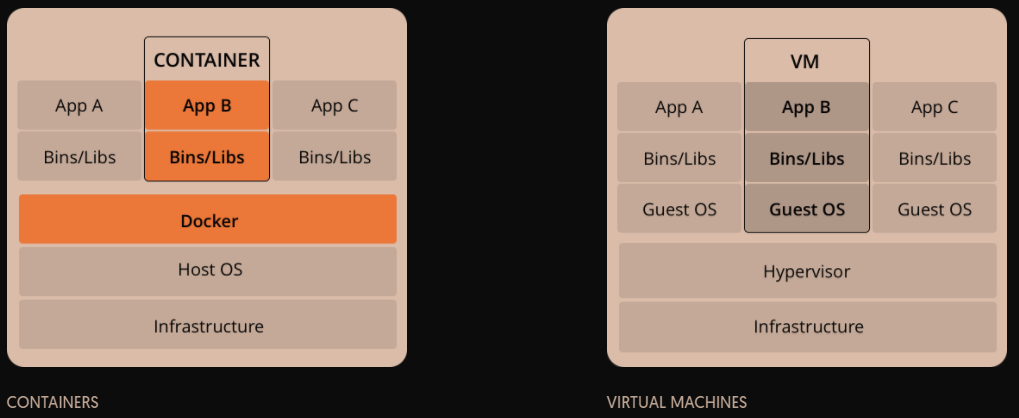
\includegraphics[width=0.7\textwidth]{dockerBlack.png}
            \attribution{\url{https://www.docker.com}}
        \end{center}
    \end{frame}

    \begin{frame}
        \frametitle{Docker Image}
        \begin{columns}
            \begin{column}{0.6\textwidth}
                \begin{itemize}
                    \item Окружение и приложение
                    \item Состоит из слоёв
                    \begin{itemize}
                        \item Все слои read-only
                        \item Образы делят слои между собой как процессы делят динамические библиотеки
                    \end{itemize}
                    \item На основе одного образа можно создать другой
                \end{itemize}
            \end{column}
            \begin{column}{0.4\textwidth}
                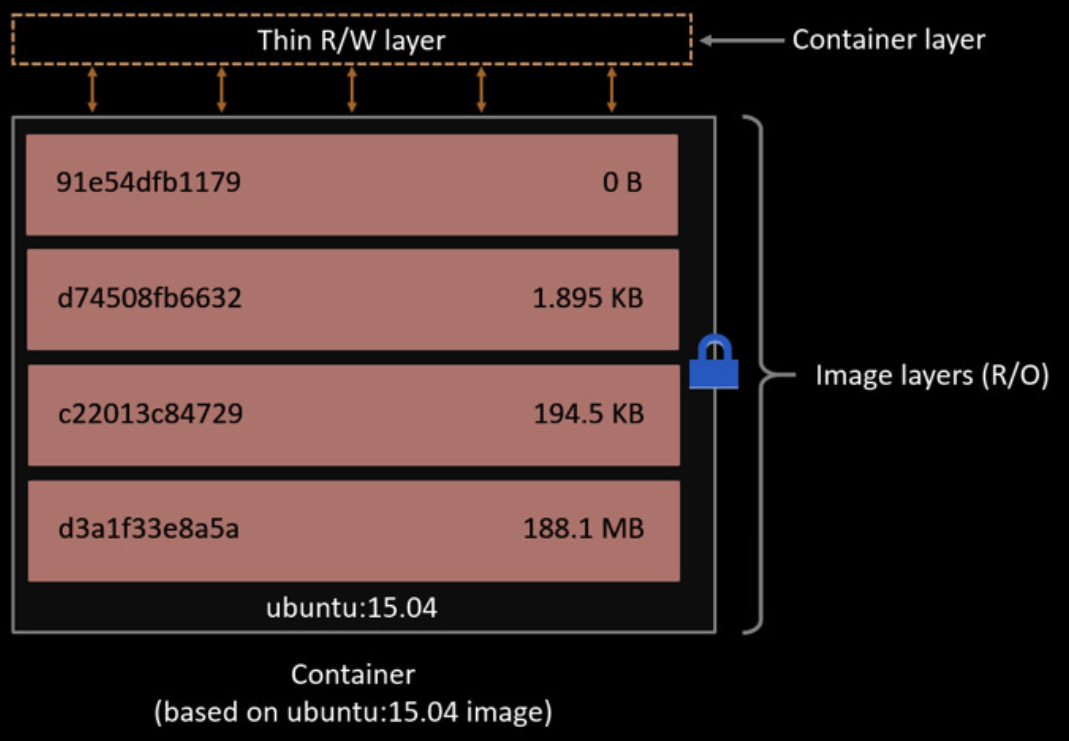
\includegraphics[width=0.9\textwidth]{dockerLayersBlack.png}
            \end{column}
        \end{columns}
    \end{frame}

    \begin{frame}
        \frametitle{Docker Container}
        \begin{columns}
            \begin{column}{0.5\textwidth}
                \begin{itemize}
                    \item Образ с дополнительным write слоем
                    \item Содержит один запущенный процесс
                    \item Может быть сохранен как новый образ
                \end{itemize}
            \end{column}
            \begin{column}{0.5\textwidth}
                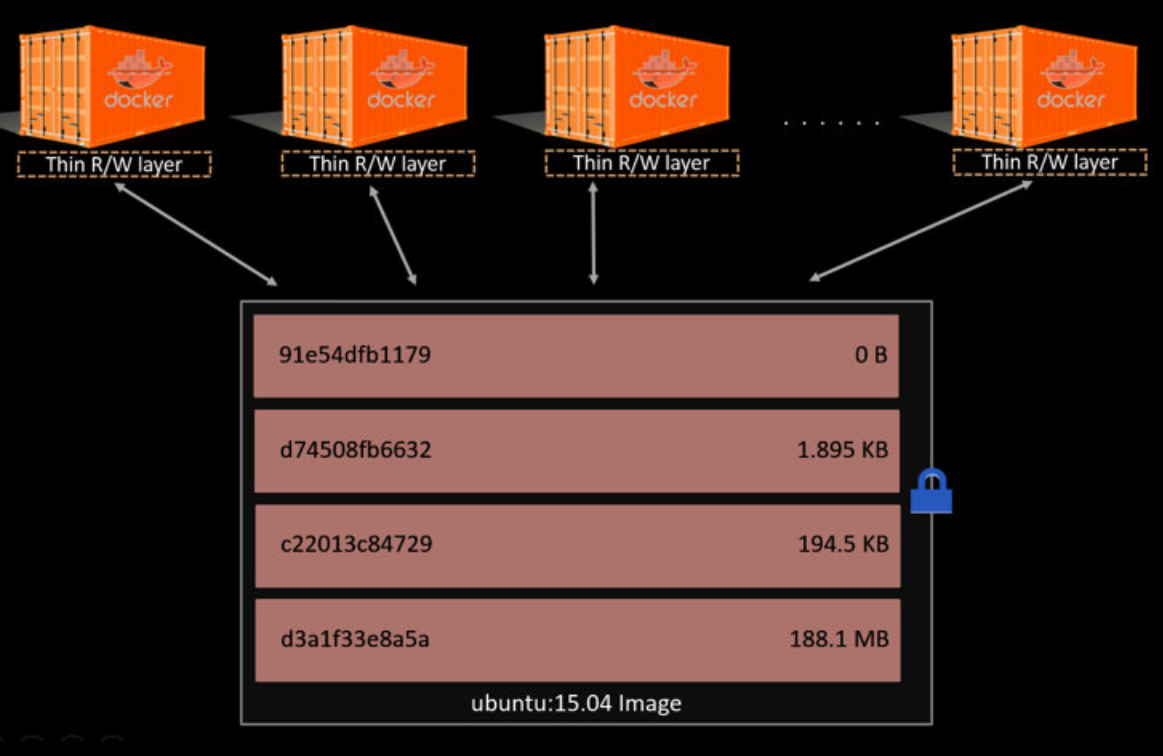
\includegraphics[width=0.9\textwidth]{dockerContainerBlack.png}
            \end{column}
        \end{columns}
    \end{frame}

    \begin{frame}
        \frametitle{DockerHub}
        \begin{columns}
            \begin{column}{0.5\textwidth}
                \begin{itemize}
                    \item Внешний репозиторий образов
                    \begin{itemize}
                        \item Официальные образы
                        \item Пользовательские образы
                        \item Приватные репозитории
                    \end{itemize}
                    \item Простой CI/CD
                    \item Высокая доступность
                \end{itemize}
            \end{column}
            \begin{column}{0.5\textwidth}
                
\includegraphics[width=0.9\textwidth]{dockerHub.png}
            \end{column}
        \end{columns}
    \end{frame}

    \begin{frame}
        \frametitle{Базовые команды}
        \begin{itemize}
            \item docker run --- запускает контейнер (при необходимости делает pull)
            \begin{itemize}
                \item -d --- запустить в фоновом режиме
                \item -p host\_port:container\_port --- прокинуть порт из контейнера на хост
                \item -i -t --- запустить в интерактивном режиме
                \item Пример: \mintinline{text}|docker run -it ubuntu /bin/bash|
            \end{itemize}
            \item docker ps --- показывает запущенные контейнеры
            \begin{itemize}
                \item Пример: \mintinline{text}|docker run -d nginx; docker ps|
            \end{itemize}
            \item docker stop --- останавливает контейнер (шлёт SIGTERM, затем SIGKILL)
            \item docker exec --- запускает дополнительный процесс в контейнере
        \end{itemize}
    \end{frame}

    \begin{frame}[fragile]
        \frametitle{Dockerfile}
        \begin{scriptsize}
            \begin{minted}{sh}
# Use an official Python runtime as a parent image
FROM python:2.7-slim

# Set the working directory to /app
WORKDIR /app

# Copy the current directory contents into the container at /app
ADD . /app

# Install any needed packages specified in requirements.txt
RUN pip install --trusted-host pypi.python.org -r requirements.txt

# Make port 80 available to the world outside this container
EXPOSE 80

# Define environment variable
ENV NAME World

# Run app.py when the container launches
CMD ["python", "app.py"]
            \end{minted}
        \end{scriptsize}
    \end{frame}

    \begin{frame}[fragile]
        \frametitle{Двухфазная сборка}
        \begin{scriptsize}
            \begin{minted}{html}
FROM mcr.microsoft.com/dotnet/aspnet:6.0 AS base
WORKDIR /app
EXPOSE 80
EXPOSE 443

FROM mcr.microsoft.com/dotnet/sdk:6.0 AS build
WORKDIR /src
COPY ["ConferenceRegistration/ConferenceRegistration.csproj", "ConferenceRegistration/"]
RUN dotnet restore "ConferenceRegistration/ConferenceRegistration.csproj"
COPY . .
WORKDIR "/src/ConferenceRegistration"
RUN dotnet build "ConferenceRegistration.csproj" -c Release -o /app/build

FROM build AS publish
RUN dotnet publish "ConferenceRegistration.csproj" -c Release -o /app/publish

FROM base AS final
WORKDIR /app
COPY --from=publish /app/publish .
ENTRYPOINT ["dotnet", "ConferenceRegistration.dll"]
            \end{minted}
        \end{scriptsize}
    \end{frame}

    \begin{frame}[fragile]
        \frametitle{Docker Compose}
        \begin{scriptsize}
            \begin{minted}{yaml}
version: "3"
services:
    web:
        image: username/repo:tag
        deploy:
            replicas: 5
            resources:
                limits:
                    cpus: "0.1"
                    memory: 50M
            restart_policy:
                condition: on-failure
        ports:
            - "80:80"
        networks:
            - webnet
networks:
    webnet:
            \end{minted}
        \end{scriptsize}
    \end{frame}

    \begin{frame}
        \frametitle{Docker Swarm}
        \begin{itemize}
            \item Машина, на которой запускается контейнер, становится главной
            \item Другие машины могут присоединяться к swarm-у и получать копию контейнера
            \item Docker балансирует нагрузку по машинам
        \end{itemize}
        \begin{center}
            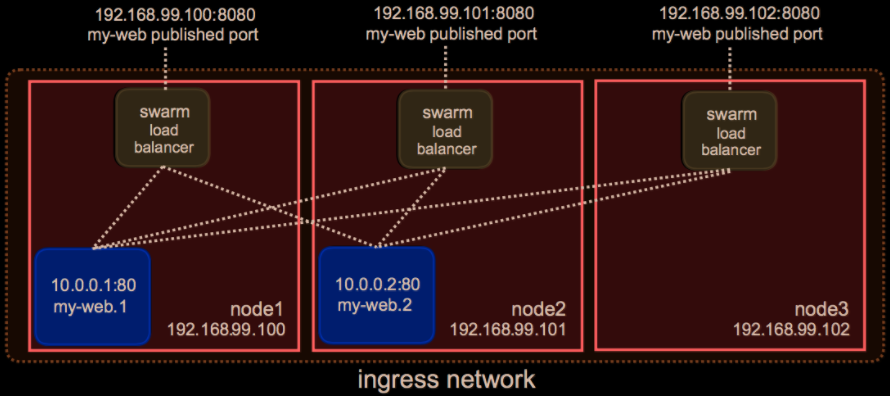
\includegraphics[width=0.7\textwidth]{swarmLoadBalancingBlack.png}
            \attribution{\url{https://www.docker.com}}
        \end{center}
    \end{frame}

    \section{Kubernetes}

    % Источник: Cloud Native DevOps with Kubernetes

    \begin{frame}
        \frametitle{Kubernetes}
        \begin{itemize}
            \item Оркестратор контейнеров
            \item Отвечает за раскидывание контейнеров по хостам, масштабирование, мониторинг и управление жизненным циклом
            \begin{itemize}
                \item Сильно продвинутый Docker Compose
            \end{itemize}
            \item Open-source, Google, Go
        \end{itemize}
        \begin{flushright}
            
\includegraphics[width=0.2\textwidth]{kubernetesBlack.png}
            \hspace{1cm}
            \attribution{\url{https://kubernetes.io/}}
        \end{flushright}
    \end{frame}

    \begin{frame}
        \frametitle{Архитектура Kubernetes}
        \begin{center}
            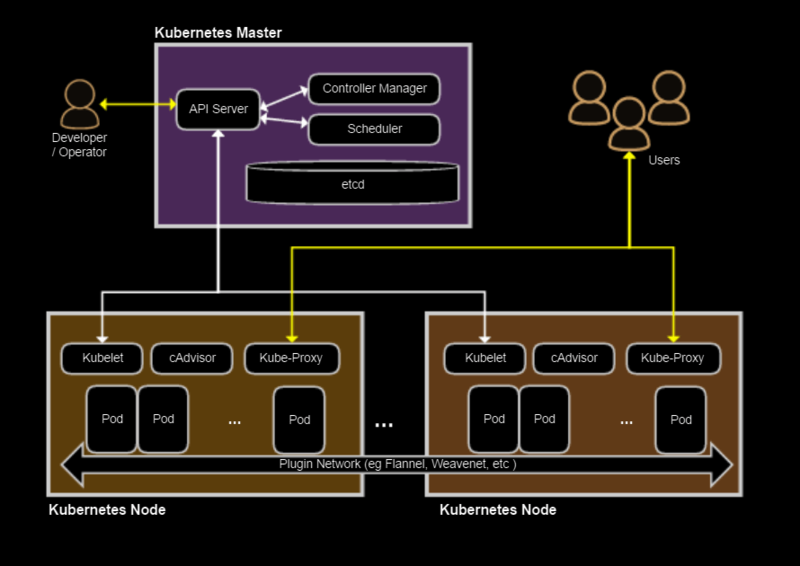
\includegraphics[width=0.8\textwidth]{kubernetesArchitectureBlack.png}
            \attribution{\url{https://ru.wikipedia.org/wiki/Kubernetes}}
        \end{center}
    \end{frame}

    \begin{frame}
        \frametitle{Объекты Kubernetes}
        \begin{center}
            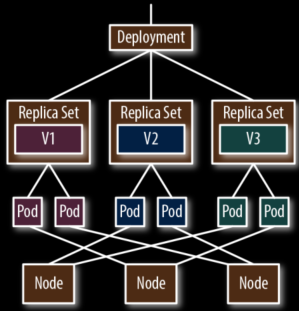
\includegraphics[width=0.4\textwidth]{kubernetesObjectsBlack.png}
            \attribution{J. Arundel, J. Domingus, Cloud Native DevOps with Kubernetes}
        \end{center}
    \end{frame}

    \begin{frame}[fragile]
        \frametitle{Deployment}
        \begin{columns}
            \begin{column}{0.4\textwidth}
                \begin{scriptsize}
                    \begin{minted}{yaml}
apiVersion: apps/v1
kind: Deployment
metadata:
  name: demo
  labels:
    app: demo
spec:
  replicas: 1
  selector:
    matchLabels:
      app: demo
  template:
    metadata:
      labels:
        app: demo
    spec:
      containers:
        - name: demo
          image: cloudnatived/demo:hello
          ports:
          - containerPort: 8888
                    \end{minted}
                \end{scriptsize}
            \end{column}
            \begin{column}{0.6\textwidth}
                Запуск:
                \begin{minted}{text}
kubectl apply -f k8s/deployment.yaml
                \end{minted}
                \attribution{J. Arundel, J. Domingus, Cloud Native DevOps with Kubernetes}
            \end{column}
        \end{columns}
    \end{frame}

    \begin{frame}
        \frametitle{Сервисы}
        \begin{center}
            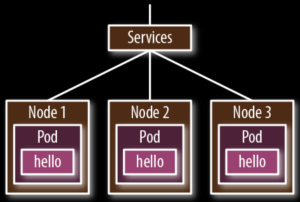
\includegraphics[width=0.4\textwidth]{kubernetesServicesBlack.png}
            \attribution{J. Arundel, J. Domingus, Cloud Native DevOps with Kubernetes}
        \end{center}
    \end{frame}

    \begin{frame}[fragile]
        \frametitle{Service}
        \begin{footnotesize}
            \begin{minted}{yaml}
apiVersion: v1
kind: Service
metadata:
  name: demo
  labels:
    app: demo
spec:
  ports:
  - port: 9999
    protocol: TCP
    targetPort: 8888
  selector:
    app: demo
  type: ClusterIP
            \end{minted}
        \end{footnotesize}
        Запуск:
        \begin{minted}{text}
            kubectl apply -f k8s/service.yaml
            kubectl port-forward service/demo 9999:8888
        \end{minted}
        \attribution{J. Arundel, J. Domingus, Cloud Native DevOps with Kubernetes}
    \end{frame}

    \begin{frame}[fragile]
        \frametitle{Рекомендации и техники}
        \begin{itemize}
            \item Конфигурация --- это код, не управляйте кластером вручную
            \item Мониторинг
                \begin{scriptsize}
                    \begin{minted}{yaml}
livenessProbe:
    httpGet:
        path: /healthz
        port: 8888
    initialDelaySeconds: 3
    periodSeconds: 3
                    \end{minted}
                \end{scriptsize}
            \item Blue/green deployment, rainbow deployment, canary deployment
            \begin{itemize}
                \item Не используйте тэг latest для Docker-образов
            \end{itemize}
            \item Используйте инструменты
            \begin{itemize}
                \item Helm, Kubernetes Dashboard и аналоги, Prometheus, Clair, Velero, ...
            \end{itemize}
            \item Метрики: Requests-Errors-Duration, Utilization-Saturation-Errors
        \end{itemize}
    \end{frame}

    \section{Облачная инфраструктура}

    \begin{frame}
        \frametitle{Облачная инфраструктура}
        \begin{itemize}
            \item Виды сервисов:
            \begin{itemize}
                \item Infrastructure as a Service
                \item Platform as a Service
                \item Software as a Service
            \end{itemize}
            \item Основные провайдеры:
            \begin{itemize}
                \item Amazon Web Services (почти 50\% рынка)
                \item Microsoft Azure (порядка 10\%)
                \item Google Cloud
                \item Всё остальное (Heroku, Yandex.Cloud, ...)
            \end{itemize}
        \end{itemize}
    \end{frame}

    % Источник: https://docs.google.com/presentation/d/13pCPuvsjATqodW5iN1qVkIU0_BEz4lYhAKTp6TbWMA0 (с разрешения Владислава Танкова)

    \begin{frame}
        \frametitle{Пример: экосистема AWS}
        \begin{itemize}
            \item Вычисления:
            \begin{itemize}
                \item EC2 (Elastic Computations)
                \item ECS (Elastic Container Service)
            \end{itemize}
            \item Сеть:
            \begin{itemize}
                \item VPC (Virtual Private Cloud)
                \item ELB (Elastic Load Balancer)
                \item API Gateway
            \end{itemize}
            \item Устройства хранения:
            \begin{itemize}
                \item EFS (Elastic File System)
                \item EBS (Elastic Block Storage)
            \end{itemize}
            \item SaaS, базы данных:
            \begin{itemize}
                \item RDS (Relational Database Service)
                \item DynamoDB
                \item ElasticSearch Service
            \end{itemize}
        \end{itemize}
    \end{frame}

    \begin{frame}
        \frametitle{Infrastructure as Code}
        \begin{columns}
            \begin{column}{0.7\textwidth}
                <<The enabling idea of infrastructure as a code is that systems and devices which are used to run software can be treated as if they, themselves, are software>> (Infrastructure as Code, Kief Morris)
                \begin{itemize}
                    \item Платформонезависимое представление инфраструктуры
                    \item Воспроизводимое развёртывание
                    \item Пример: Terraform
                \end{itemize}
            \end{column}
            \begin{column}{0.3\textwidth}
                \begin{center}
                    
\includegraphics[width=0.9\textwidth]{terraformLogoBlack.png}
                \end{center}
            \end{column}
        \end{columns}
    \end{frame}

\end{document}
